\documentclass[12pt, a4paper]{report}
\usepackage[utf8]{inputenc}
\usepackage[T1]{fontenc}
\usepackage[polish]{babel}
\usepackage{titling}
\usepackage{graphicx}
\usepackage{lmodern}
\usepackage[a4paper, margin=1in, top=0.5in, bottom=1in]{geometry}
\usepackage{footnote}
\usepackage{float}

\setlength{\parindent}{1cm}
\setlength{\parskip}{0cm}

% notes:
% - In polish we write titles of projects, chapters, sections with only first letter of first word large

\title{
``Sprawozdanie z projektu BigData\\ 
Predykcja cen samochodów używanych''
}
\author{
    Mateusz Grzybek 240678\\
    Kamil Młynarczyk  240757
}
\date{\today}

\begin{document}

%Title page definition
\begin{titlepage}
    \centering

    % University information
    {\Huge Politechnika Łódzka \\[0.5cm]}
    {\Large Wydział Elektrotechniki Elektroniki Informatyki i Automatyki \\[0cm]}
    
\includegraphics[width=0.5\textwidth]{images/university_logo}
    {\\[0cm] sem, zimowy, r ak. 2024/2025 \\[1cm]}
    
    % Project information
    {\Large \textbf{
        Sprawozdanie z projektu BigData\\ 
        „Predykcja cen samochodów używanych” \\[0.2cm]
    }}
    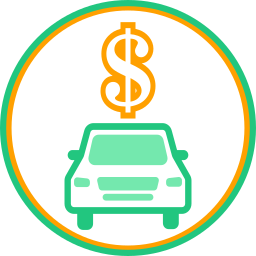
\includegraphics[width=0.3\textwidth]{images/project_logo.png}
    {\\[0.3cm]}
    % Author information
    {\Large Mateusz Grzybek 240678 \\[0.2cm] Kamil Młynarczyk 240757 \\[1cm]}

    % Publication date
    {\Large \today}
\end{titlepage}

% Table of contents
\tableofcontents
\thispagestyle{empty}
\newpage

% chapter 1 - Introduction
\chapter{Wstęp}
\section{Założenia projektowe}
Celem projektu jest zaimplementowanie aplikacji webowej pozwalającej użytkownikom na predykcję 
ceny używanego samochodu na podstawie dostarczonego przez niego zestawu cech. Tematyka projektu
daje możliwość wykorzystania różnorodnych technologii z dziedziny uczenia maszynowego, rozwoju
aplikacji webowych, komunikacji pomiędzy serwisami,architektury oprogramowania oraz bierania i 
przetwarzania danych. W celu zrealizowania przewidywanych funkcjonalności, aplikacja została
podzielona na cztery komponenty, każdy z nich odpowiedzialny za realizację innego aspektu
aplikacji.
\section{Komponenty}
\begin{itemize}
    \item Aplikacja kliencka --- Interfejs graficzny użytkownika.
    \item Pośrednik --- Komponent pośredniczący w komunikacji pomiędzy aplikacją kliencką i serwisem predykcyjnym
    \item Komponent komunikacyjny --- Komponent zawierający szyny danych, które są wykorzystywane do dostarczania i odbierania informacji od serwisu predykcyjnego
    \item Serwis predykcyjny --- Komponent dokonujący predykcji na podstawie dostarczonych danych, z wykorzytaniem nauczonego modelu.
\end{itemize}
\section{Wykorzystane technologie}
\begin{itemize}
    \item Java --- Obiektowy język programowania.
    \item SpringBoot --- Framework dla języka Java nastawiony na wytwarzanie aplikacji webowych i mikroserwisów
    \item Gradle --- Narzędzie do automatyzacji budowania projektów.
    \item React --- Framework JavaScript do tworzenia interfejsów użytkownika w oparciu o komponenty.
    \item Docker --- Narzędzie do tworzenia, uruchamiania i zarządzania aplikacjami w izolowanych środowiskach zwanych kontnerami.
    \item Docker Compose --- Narzędzie usprawniające zarządzanie wieloma kontenerami jednocześnie.
    \item Python --- Język skryptowy. 
    \item Apache Spark --- Framework do sprawnego przetwarzania zbiorów danych w pamięci.
    \item Apache SparkML --- Moduł Apache Spark przeznaczony do uczenia maszynowego.
    \item Apache Kafka --- Platforma przetwarzania danych w czasie rzeczywistym.
    \item Apache Zookeeper --- Usługa koordynacyjna systemów rozproszonych.
\end{itemize}

\chapter{Aplikacja kliencka}
\section{Opis}
Aplikacja kliencka stanowi pojedynczą stronę dostępną za pośrednictwem przeglądarki,
udostępnianą pod adresem \textbf{localhost}\footnote{loopback address --- adres pętli zwrotnej, który jest wykorzystywany do komunikacji urządzenia z samym sobą.},
na porcie \textbf{9091}. Strona zawiera informacje związane z aplikacją oraz pola do wprowadzania wartości,
na podstawie których następnie dokonywana jest predykcja ceny samochodu. Aplikacja łączy się z komponentem
middleware za pośrednictwem protokołu \textbf{HTTP}\footnote{HyperText Transfer Protocol --- protokół komunikacyjny używany do przesyłania danych w sieci.}
 w architekturze 
\textbf{REST}\footnote{Representational State Transfer --- architektura komunikacji oparta o protokół HTTP
    definiujący sposoby identyfikacji i manipulacji zasobami za pomocą zapytań HTTP.}.\@
\section{Widoki aplikacji}
\subsection{Strona}
\begin{figure}[H]
    \centering
    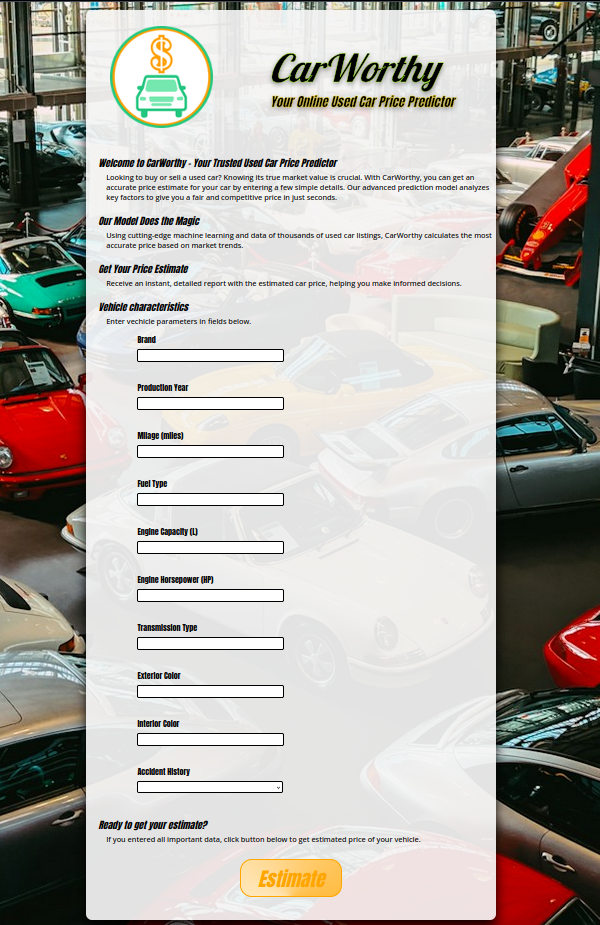
\includegraphics[width=0.9\textwidth]{images/page_view}
    \caption{Widok strony}
\end{figure}
\subsection{Okno z ceną}
\begin{figure}[H]
    \centering
    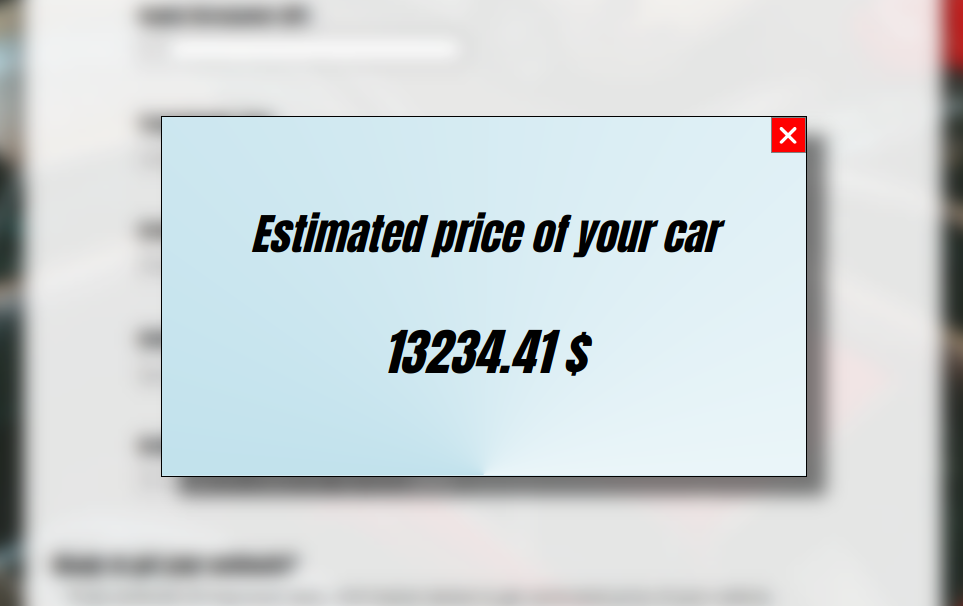
\includegraphics[width=0.9\textwidth]{images/price_view}
    \caption{Widok okna z ceną}
\end{figure}
\subsection{Okno z błędem}
\begin{figure}[H]
    \centering
    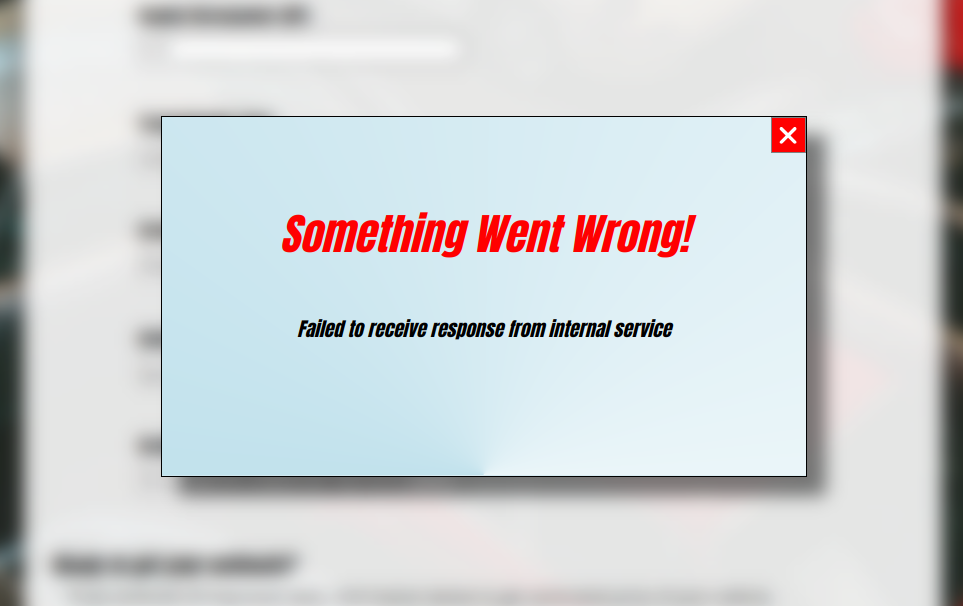
\includegraphics[width=0.9\textwidth]{images/error_view}
    \caption{Widok okna z błędem}
\end{figure}

\chapter{Komponent pośredniczący i komunikacyjny}
\section{Komponent pośredniczący}
\subsection{Opis}
Komponent pośrediczący pełni rolę pośrednika pomiędzy aplikacją kliencką i serwisem predykcyjnym.
Otrzymywane od \textbf{frontendu}\footnote{Część aplikacji, z którą użytkownik wchodzi w bezpośednią interakcję, w tym wszystko co widzi oraz elementy wizualne i interaktywne.}
dane w formie \textbf{JSON}\footnote{JavaScript Object Notation --- format danych zapewniający kompaktowe rozmiary i jest czytelny dla ludzi i maszyn.}
są w tym komponencie przetwarzane na wiadomości w formacie odpowiadającym wejściu modelu, z uwzględnieniem procesu \textbf{kodowania liczbowego}\footnote{
Technika zamiany wartości danych tekstowych na wartości liczbowe, poprzez przypisanie unikalnej liczby każdej unikalnej wartości tekstowej.
} pól. Otrzymane
w tym procesie wiadomości zapisywane są na \textbf{temat}\footnote{Podstawowy komponent Apache Kafka służący do kategoryzacji napływających wiadomości.}
 wejściowy Kafki. Pośrednik jest również odpowiedzialny za odczytywanie danych z tematu wyjściowego i
przekazywanie uzyskanych z nich informacji do klienta.
\section{Komponent komunikacyjny}
\subsection{Opis}
Komponent komunikacyjny odpowiedzialny jest za transport danych pomiędzy komponentem pośredniczącym i serwisem predykcyjnym.
Wykorzystuje w tym celu skonteneryzowany \textbf{broker}\footnote{Serwer Apache Kafka zawierający dane należace do tematów i partycji, na które może być podzielony temat}
wiadomości Apache Kafka wraz z dwoma tematami input oraz output, wykorzystywanych
odpowiednio do gromadzenia danych odczytywanych przez serwis predykcyjny i gromadzenia danych odczytywanych przez pośrednika.
Do zarządzania brokerem wykorzystywany jest Apache Zookeeper.

\chapter{Diagramy}
\section{Diagram przypadków użycia}
\begin{figure}[H]
    \centering
    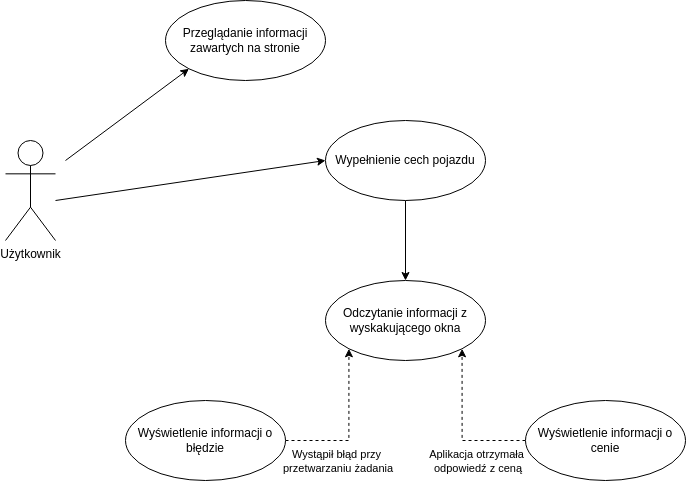
\includegraphics[width=1\textwidth]{diagrams/use_case_diagram.png}
    \caption{Przebieg interakcji użytkownika z aplikacją}
\end{figure}
\section{Diagram sekwencji zdarzeń}
\end{document}